\section{Final results}

\subsection{Absolute Execution Times}

The first graph illustrates the absolute execution time for the MKL, BLIS, and AOCL implementations, in both single-core and multi-core modes.

\begin{figure}[h!] % [h!] forces the figure to appear here
    \centering
    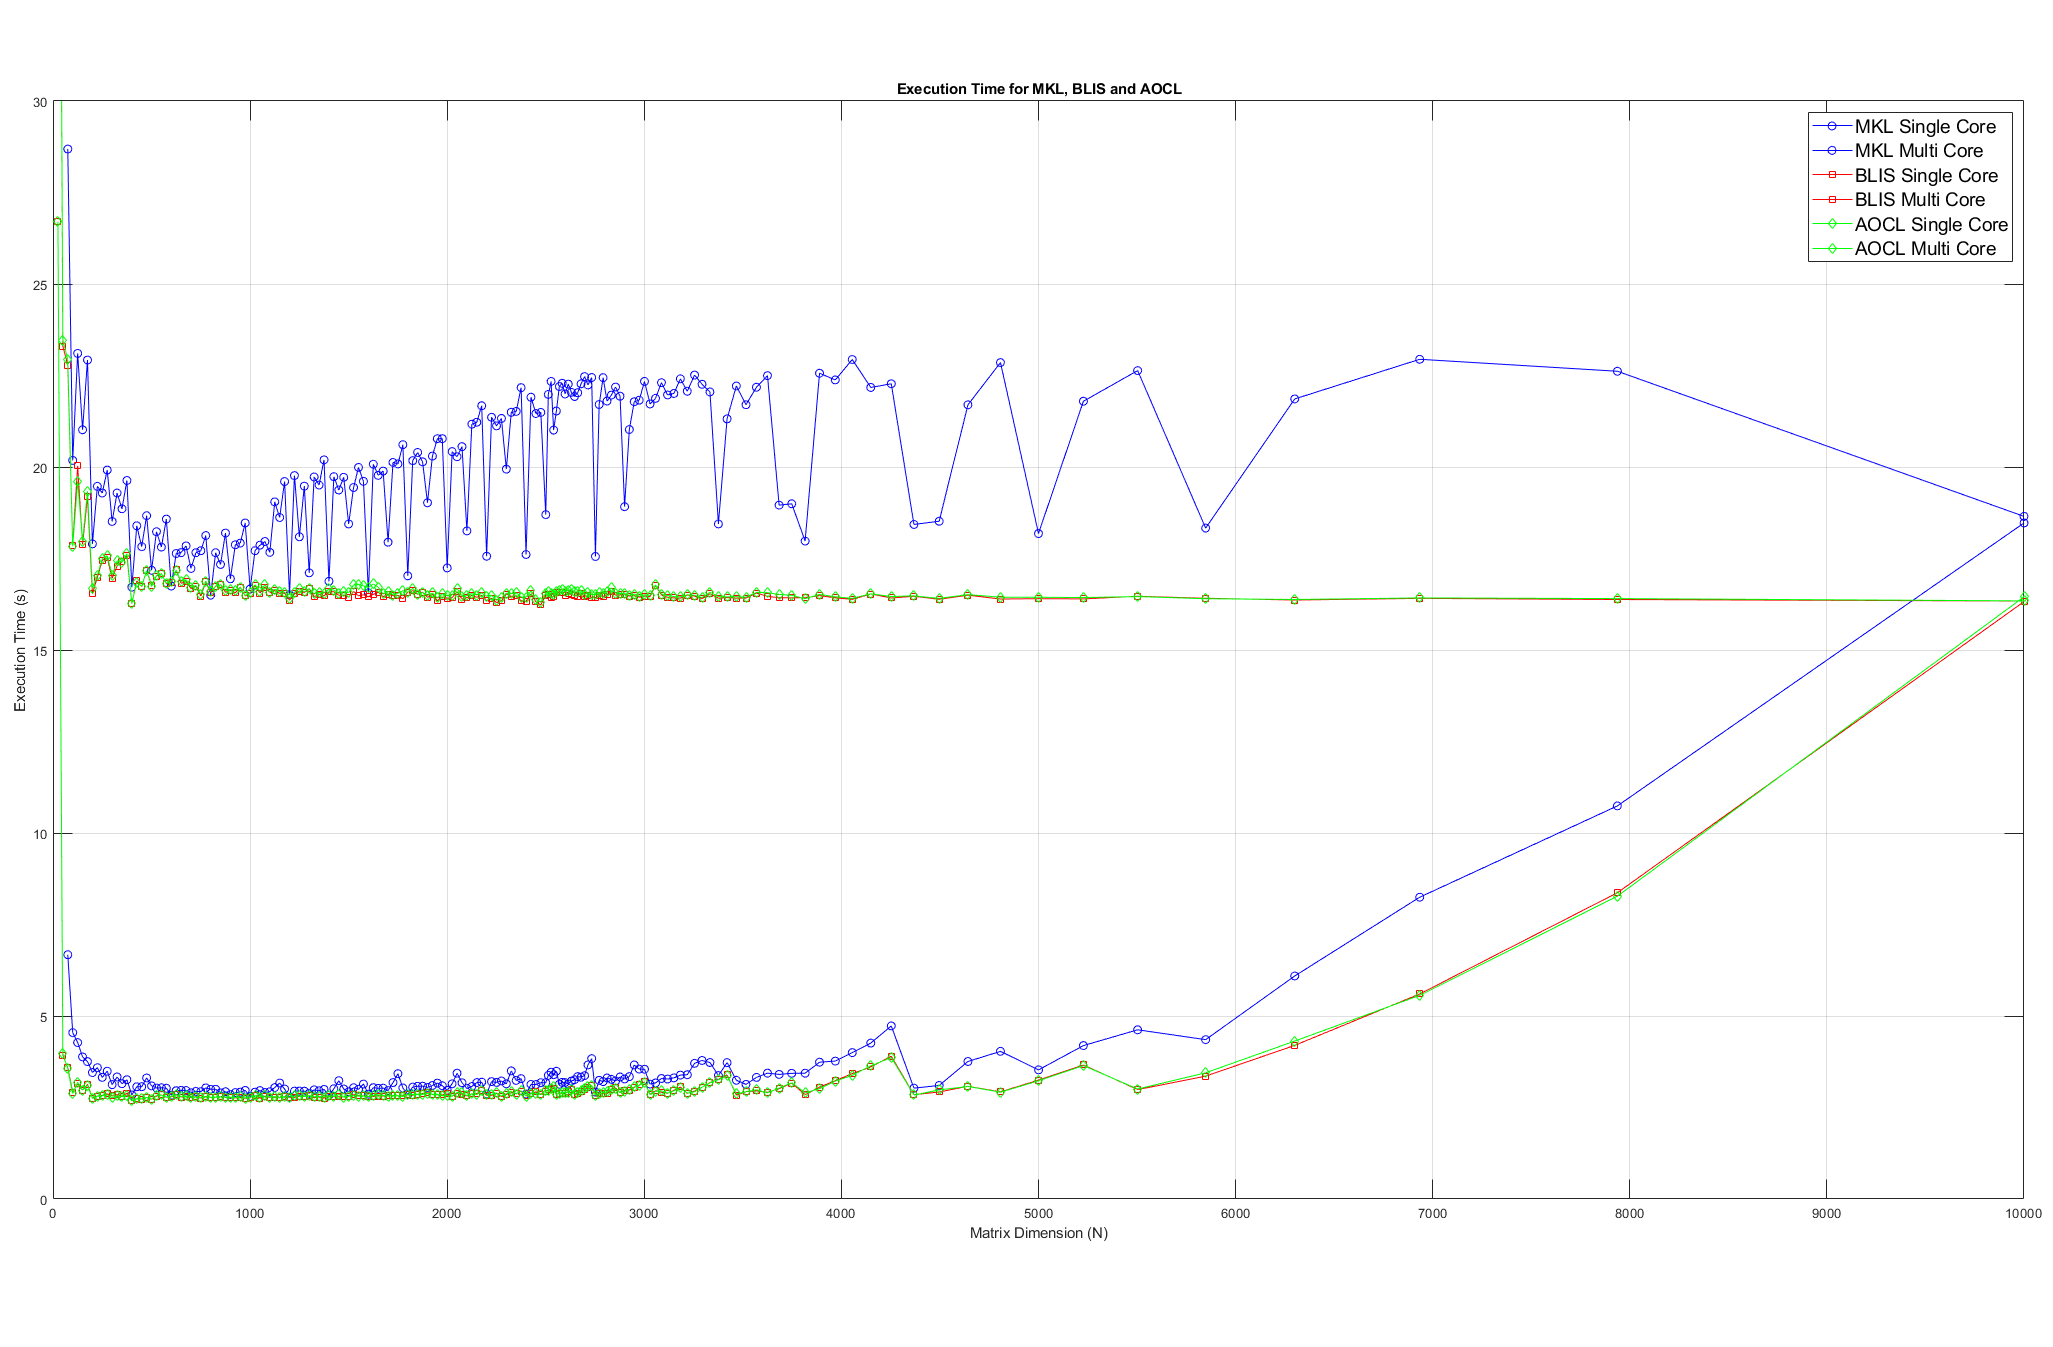
\includegraphics[width=\linewidth]{Figures/Imagenes/Final1.png} % Adjusts the image to the width of the line
    \caption{}
\end{figure}

\begin{itemize}
    \item \textbf{MKL:} Intel's MKL library, while known for its performance on Intel processors, delivered unexpected results on the AMD Ryzen 5 5600X. The single-core performance, in particular, displayed anomalies. One plausible reason could be the library's optimization towards Intel architectures, which might not translate as effectively on AMD platforms. However, its multi-core capability does show some improvement.
    
    \item \textbf{BLIS:} BLIS showcased a consistent performance across both single-core and multi-core modes. Its execution times provide a stable benchmark, demonstrating adaptability across different processor architectures.
    
    \item \textbf{AOCL:} Given that AOCL is a fork of BLIS, their results mirroring each other was expected. This matching performance in both single-core and multi-core modes underscores AOCL's roots in the BLIS codebase.
\end{itemize}



\subsection{Speed Up: Comparison of Single Core vs Multi Core}

The speed-up factor reflects the efficiency with which each implementation harnesses parallelism when activating multiple cores. The second graph underscores the intricacies of the interplay between single-core anomalies and perceived multi-core speed-up benefits.

\begin{figure}[h!] % [h!] forces the figure to appear here
    \centering
    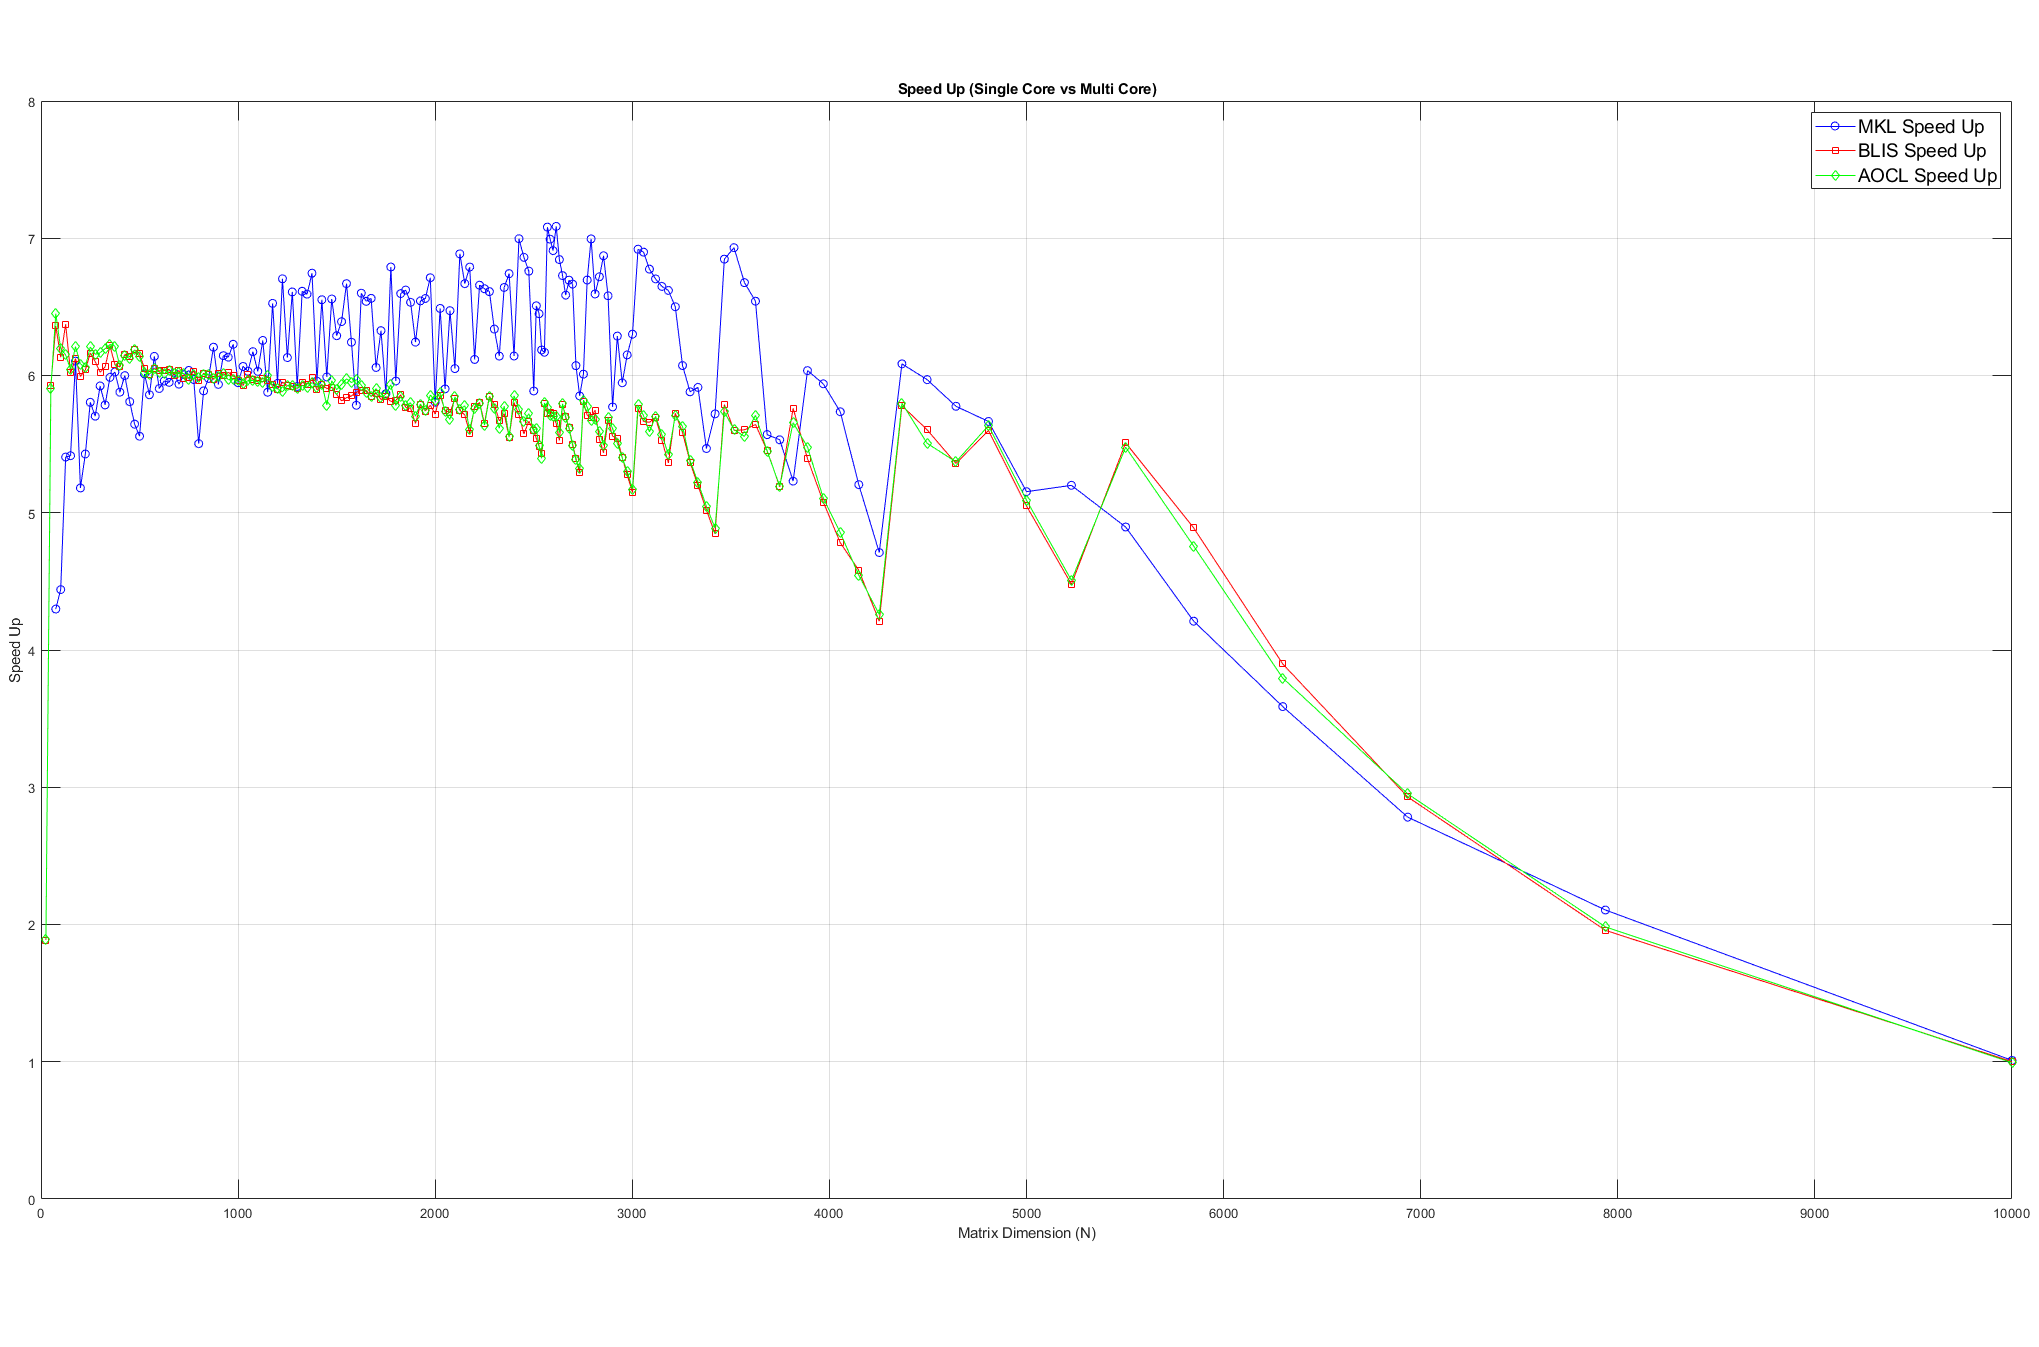
\includegraphics[width=\linewidth]{Figures/Imagenes/Final2.png} % Adjusts the image to the width of the line
\end{figure}
\vspace{-1em}
\begin{itemize}
    \item \textbf{MKL:} With the unexpected behavior in single-core performance already commented, MKL seems to present an exaggerated speed-up, surpassing theoretical limits. This is misleading, as the poor single-core performance artificially boosts the speed-up metric when transitioning to multi-core. Maximum speed-up would be 6, given the AMD Ryzen 5 5600X's 6 cores.
    
    \item \textbf{BLIS and AOCL:} Both BLIS and AOCL showcase a more uniform behavior, aligned with anticipated speed-ups on a 6-core processor. However, as the matrix dimension \( N \) increases, there's a notable decline in the speed-up. This reduction is largely due to the operation loop running over the variable \texttt{TIMES}. As \( N \) grows, \texttt{TIMES} diminishes to maintain a consistent operation count. When \texttt{TIMES} drops below the number of cores, some cores remain idle during the multi-core test, as there isn't enough work to parallelize across all cores. This is particularly evident with \( N=10000 \) where the speed-up approaches 1, indicating that only a single core is actively computing.

\end{itemize}


\subsection{Final Comparison of Execution Times}

The graph below contrasts the execution times of multi-core CPU and GPU matrix computations. GPU tests were made with and without the data transfer between GPU and CPU (the memory transfer is set for every operation, being the worst case scenario possible).

\begin{figure}[h!] % [h!] forces the figure to appear here
    \centering
    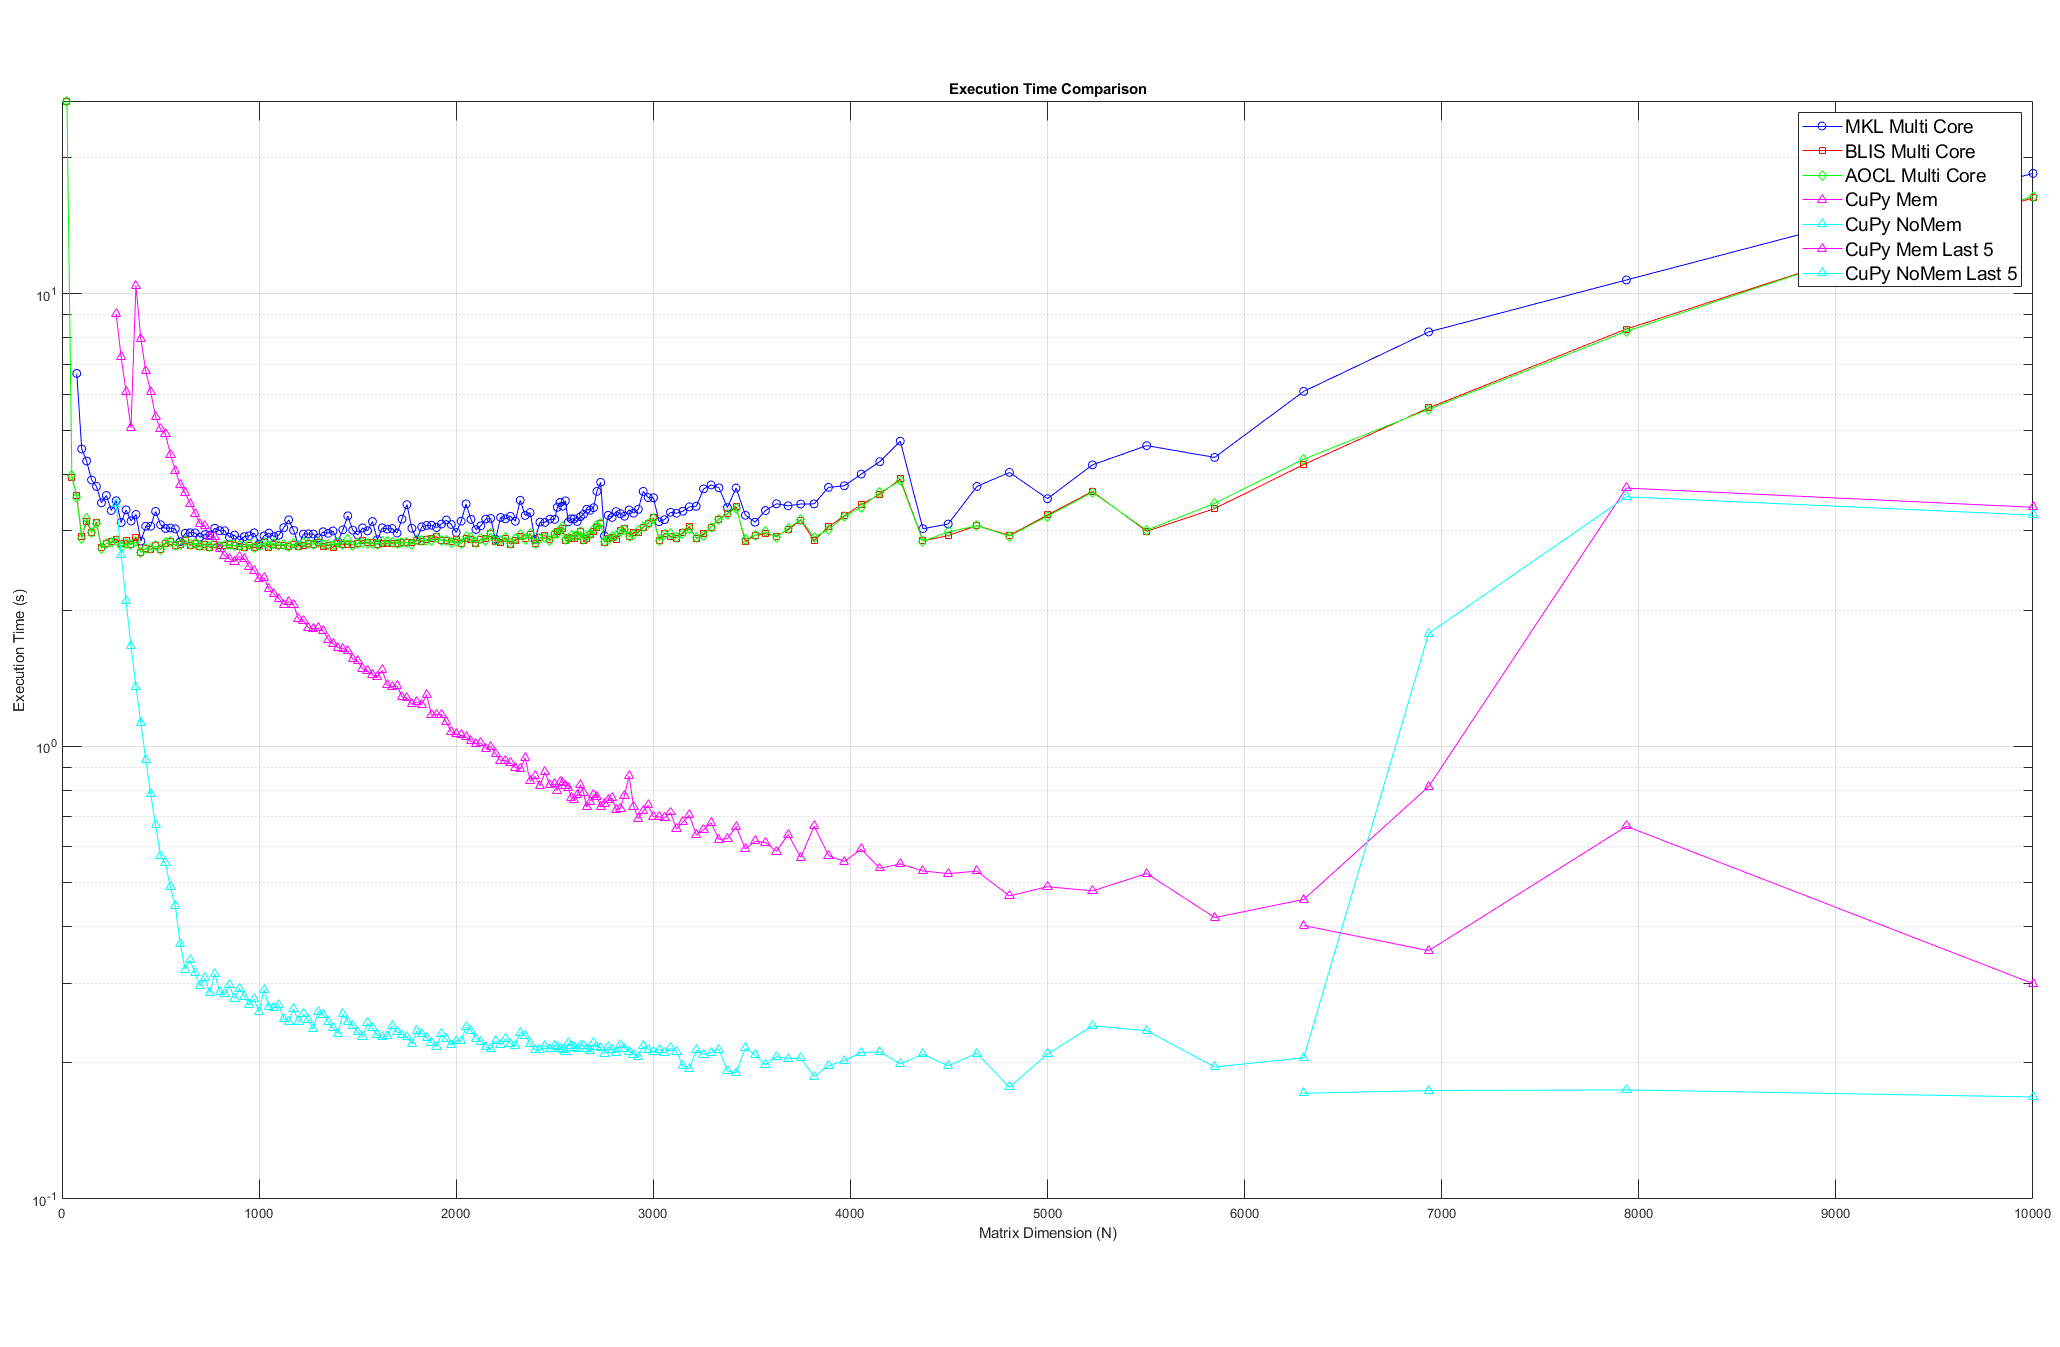
\includegraphics[width=\linewidth]{Figures/Imagenes/Final3.png} % Adjusts the image to the width of the line
\end{figure}

\vspace{-1em}

\textbf{Garbage collector on Python:} The garbage collector impacts CuPy execution times. In the final tests for CuPy, two patterns are observed: one set of results shows increased execution times due to the garbage collector, while the other set, which only includes the last 5 tests, shows improved times without the garbage collector's interference.

\textbf{Memory access:} Even in conditions where memory is copied for every AxB = C operation, GPU performance using CuPy surpasses multi-core CPU implementations by a substantial margin, completing tasks almost an order of magnitude faster.

\subsection{Conclusion}

The analysis highlights the performance differences between multi-core CPU and GPU matrix computation methods. These results are essential for making informed decisions regarding computational methods. Given the GPU's superiority, even under sub-optimal conditions, it suggests a trend towards favoring GPU-based operations in future computational tasks.




